\documentclass{article}
\usepackage{amsmath,amssymb}
\usepackage{graphicx}
\usepackage{bm}
\usepackage[numbers,sort&compress]{natbib}
\usepackage{color}
\usepackage{tabularx}

\title{The binary liquid model for gravity-driven microchannel simulations}
\date{\today}
\newcommand{\Ca}{\mathrm{Ca}}
\newcommand{\todo}[1]{{\color{red}#1}}
\begin{document}

\maketitle

\begin{abstract}
This work shows that the free-energy binary liquid lattice Boltzmann method is able to
reproduce the gravity driven microchannel flow of an air bubble through liquid. In the low capillary
number
$\Ca$ regime (defined in Eq. \ref{capillary:number:definition}), the flow is thoroughly described by
Bretherton \cite{bretherton},
with the deposition film thickness proportional to $\Ca^{2/3}$. However, there are deviations
from the Bretherton correlations for $Ca\geq 0.005$, studied experimentally and numerically. This
work aims to examine the lattice Boltzmann binary liquid model feasibility to obtain valid results
for an air bubble flow in liquid for a range of $Ca$ number. The binary
liquid model is a continuous-interface multiphase model, which raises
the question of how to properly resolve the interface in comparison with the film thickness.
It was found that the film interface needs to be as $50$
percent in comparison with the film thickness for simulation to give convergent results. While
the convergency criteria is fulfilled the results are of good comparison with the
numerical simulations of \citet{giavedoni-numerical} in the range of $Ca$ from $0.01$ to $1$. 
\end{abstract}


\section{Introduction}
The Taylor/Bretherton \cite{bretherton} flow describes the flow of long bubbles in
microchannels. It was found that the front meniscus film width is proportional
to $\Ca^{2/3}$ for capillary numbers less than $0.003$, where the capillary number is defined as:
\begin{equation}
\label{capillary:number:definition}
Ca=\frac{\mu_{liq} U_{bubble}}{\gamma},
\end{equation}
where $\mu_{liq}$ is the liquid viscosity, $U_{bubble}$ is a propagation bubble velocity, and
$\gamma$ is the surface tension between air and liquid.
While there are number
of works which simulate the Bretherton problem with the boundary value method
\cite{ingham-plates,heil-bretherton}, those methods are of limited applicability for problems
involving complex geometries, free interface motion or for problems involving coalescence and/or
droplet breakup. The continuous interface models are more flexible for those kind of simulations.
However, if the interface is spread over several grid nodes, the question of
proper film width resolution in comparison with the interface arises.  This work
concentrates on resolving the parameter range of the binary liquid lattice
Boltzmann method to validate it in the range of capillary numbers.

The lattice Boltzmann method has emerged as a successful method to simulate
a wide variety of phenomena including hydrodynamics \cite{yu}, thermal flows
\cite{karlin-minimalmodels}, microflows \cite{ansumali-small-knudsen},
ferrofluids \cite{kuzmin-aniso}, and multiphase flows
\cite{swift,Shan-chen:extended}. Thanks to its kinetic nature, LBM as a particle
method easily tackles complex geometries andallows for incorporation of
physical phenomena on the microscopic level, as in the case in multiphase models. Most
multiphase lattice Boltzmann models \cite{swift, Shan-chen:extended} resolve
the interface in a continuous way. Such a representation
brings issues with film thickness resolution versus interface
resolution. In other words, when it comes to the resolution of the film
thickness the diffusive interface should be resolved in such a way as to have
negligible effect on the physics of the film.

This work examines the binary liquid free-energy LB model \cite{swift}. The
model simulates two liquids with the assumption of uniform overall
density. While the classical Bretherton problem is stated for air and liquid, which are of largely
different densities and viscosities, it was indicated \cite{bretherton} that inertia effects were
neglected. Moreover, the results of \citet{giavedoni-numerical} and \citet{heil-bretherton} show
negligible Reynolds number effect on the film thickness for the range of Reynolds numbers.
Therefore, the governing factor for microchannel flows is not the densities ratio, but the
viscosities ratio. Moreover, the results based on the uniform density, as in the case of the LBM
binary liquid model, are of good comparison with other simulations
\cite{giavedoni-numerical,heil-bretherton} taking into the account inertia effects. 

The goal of this paper is to give an answer as to how to choose the
binary liquid model parameters, the viscosities ratio and the grid
resolution, in order to obtain correct film thicknesses.

The paper is organized as follows.  First, we briefly
explain the binary liquid lattice Boltzmann model and summarize the literature
for the Bretherton problem. Then, the parameters involved in the
simulation are examined and presented in the results section. The paper is
concluded with a summary of the main findings.

\section{Bretherton bubble flow}
Bretherton \cite{bretherton} studied a long bubble
moving in a tube filled with liquid. It was found that the deposition film width
is proportional to $\Ca^{2/3}$ in the range of small capillary numbers. Later on
it was realized \cite{wong-films,wong-pressure} that the film deposition
is proportional to $\Ca^{2/3}$ only in the specific region behind the front meniscus and
that the film width
varies over the bubble length for bubbles of finite length. Numerical
simulations \cite{giavedoni-numerical} and experimental studies
\cite{kreutzer-pressure-drop} showed as well a Reynolds number dependence, and
a deviation from the $\Ca^{2/3}$ rule for capillary numbers larger than $0.003$.
To be able to predict consistently the flow pattern for capillaries in
different ranges of parameters, simulations have been developed and are typically validated with the
small capillary numbers Bretherton problem.

There are a number of numerical methods which
were used for the simulation of the Taylor/Bretherton flow.
\citet{vanbaten-circular} studied the mass transfer and film
thickness for rising bubbles in a circular capillary using the finite volume method.
\citet{kreutzer-pressure-drop} used the finite volume method as well to perform
simulations of a circular capillary for a number of different
Reynolds and capillary numbers. \citeauthor{wong-films} \cite{wong-films,wong-pressure} studied
three-dimensional bubbles in
polygonal capillaries and showed the derivations of different shapes in the
slug crossections and menisci appearance.
\citet{heil-bretherton,ingham-plates} studied air finger propagation in
a two-dimensional channel for a range of Reynolds and capillary
numbers using finite element method. \citet{giavedoni-numerical} performed crossvalidation of the
finite element solution developed by them with previously published results.
The solution is available for circular and planar cases.

While the applicability of other methods is well established for the
simulation of the Bretherton/Taylor problem, this is not the case for
the lattice Boltzmann method. A thorough parameter study for this approach
has not yet been done to the best of the authors' knowledge.

One should acknowledge the works of \citet{pagonabarraga-fingers} on menisci
in thin films for fingering phenomena. \citet{sehgal-microchannel} performed lattice Boltzmann
simulations of two-dimensional channel flows for larger capillary numbers, and
the authors found discrepancies with the classical Bretherton theory, which
is limited to the low capillary number regime \cite{giavedoni-numerical}.

To resolve the interface on a fine level for capillary numbers less than
$0.003$ is computationally intensive even in the two-dimensional case
(the amount of memory necessary to perform the simulation is on the order
of tens or hundreds of gigabytes).  This work is therefore based on a
comparison with the already established results, which were themselves
validated for the Bretherton bubble flow.  In this paper, we present
recipes for the initialization of the simulations and discuss optimal
parameter ranges for the binary liquid LB model.

\section{Lattice Boltzmann binary liquid model}
The lattice Boltzmann equation (LBE) operates on a rectangular grid representing the
physical domain. It utilizes
probability distribution functions (also known as particle populations)
containing information about
macroscopic variables, such as fluid density and momentum. LBE consists of
two parts: a local collision step, and a propagation step which transports
information from one node to another in certain
directions specified by the discrete velocity set.
The LBE is typically implementated as follows:
\begin{equation}
\label{standard:implementation}
\begin{aligned}
&f_i^{*}(\bm{x},t)=\omega f_i^{eq}(\bm{x},t)-(1-\omega) f_i(\bm{x},t) +
F_i,&&\text{ collision step}\\
&f_i(\bm{x}+\bm{c_i},t+1)=f_i^{*}(\bm{x},t),&&\text{ propagation step}, 
\end{aligned}
\end{equation}
where $F_i$ is the external force population. The binary fluid LB model is
based on a free-energy functional \cite{swift,landau}, and operates with two
sets of populations: one to track the pressure and velocity fields, and the
other to represent the phase field.

The model we use in this work is a two-dimensional nine-velocity (D2Q9) model,
with equilibrium populations \cite{pooley-contact}:
\begin{equation}
\begin{aligned}
&f_i^{eq}&&=w_i 
\biggl(3
p_0 - k \phi \Delta \phi
+\frac{u_{\alpha}c_{i\alpha}}{c_s^2}+\frac{Q_{i\alpha\beta}u_{\alpha } u_ {
\beta}}{2 c_s^4}\biggr)\\
&&&+k\bigl(w_i^{xx} (\partial_x \phi)^2+w_i^{yy} (\partial_y \phi)^2 +w_i^{xy} \partial_x
\phi \partial_y \phi \bigr), i=1\div8\\
&f_0^{eq}&&=\rho-\sum_{i\neq0}{f_i^{eq}}\\
&g_i^{eq}&&=w_i\left(\Gamma \mu + \frac{\phi c_{i\alpha} u_{i\alpha}}{c_s^2}+\phi^m
\frac{Q_{i\alpha\beta}u_{\alpha}u_{\beta}}{2 c_s^4}\right), i=1\div8 \\
&g_0^{eq}&&=\phi-\sum_{i\neq0}{g_i^{eq}}\quad,
\end{aligned}
\end{equation}
where $\Gamma$ is the mobility parameter; the chemical potential
$\mu=-A\phi+A\phi^3-k\Delta\phi$; $k$ is related to the surface
tension; $A$ is a parameter of the free-energy model  The bulk pressure
is expressed as $p_0=c_s^2 \rho +A (-0.5 \phi^2+0.75 \phi^4)$. 
Parameters speficic to the D2Q9 grid are the weights
$w_i=\left\{\frac{4}{9},\frac{1}{9},\frac{1}{9},\frac{1}{9},\frac{1}{9},
\frac{1}{36},\frac{1}{36},\frac{1}{36},\frac{1}{36}\right\}$, and the tensor
$Q_{i\alpha\beta}=c_{i\alpha} c_{i\beta} - c_s^2 \delta_{\alpha\beta}$ with
the sound speed parameter $c_s^2=1/3$.  The weights related to the
inclusion of the surface tension coefficient into the equations are as follows:
$w^{xx}_{1-2}=w^{yy}_{3-4}=1/3$, $w^{xx}_{3-4}=w^{yy}_{1-2}=-1/6$,
$w^{xx}_{5-8}=w^{yy}_{5-8}=-1/24$, $w^{xy}_{1-4}=0$, $w^{xy}_{5-6}=1/4$ and
$w^{xy}_{7-8}=-1/4$. The system can be shown to restore the macroscopic
fluid equations as:
\begin{equation}
\begin{aligned}
&\partial_t \rho+ \partial_{\alpha} \rho u_{\alpha}=0\\
&\rho\left(\partial_t+u_{\beta}\partial_{\beta}\right) u_{\alpha}=
-\partial_{\alpha}P_{\alpha \beta} +
\nu\partial_{\beta}\left(\partial_{\alpha}u_{\beta}+\partial_{\beta} u_{\alpha}\right)\\
&\partial_t \phi + \partial_{\alpha} \phi u_{\alpha}=M \partial^2_{\beta\beta} \mu,
\end{aligned}
\label{binary:fluid:system}
\end{equation}
where $\nu=c_s^2 (\tau-1/2)$ is the viscosity and
$M=\Gamma(\tau_{\phi}-1/2)$ is the mobility parameter. The system allows the separation of the liquid
phase with $\phi=1$ and a so-called gas phase with $\phi=-1$. The
relaxation time is taken as linearly dependant on the relaxation
times $\tau_{\mathrm{gas}}$ and $\tau_{\mathrm{liq}}$:
$\tau=\tau_{\mathrm{gas}}+\frac{\phi+1}{2}\tau_{\mathrm{liq}}$.
The surface tension in the framework of the binary liquid model is $\sqrt{\frac{8 k A}{9}}$.

\section{Lattice Boltzmann benchmark}
To properly simulate and to compare simulation results with the data
published in the literature, one needs to design a numerical benchmark addressing
the following challenges for the lattice Boltzmann method:
\begin{itemize}
 \item The diffusive nature of the interface in the multiphase model should not
influence the film width results. This is obviously achieved only for certain
resolutions of the interface in comparison with the film width. The same applies to spurious
currents arising from surface tension discretization which
can influence mass transfer in the thin film, thereby compromising the
overall solution. Therefore the diffusive interface should be of nengligible influence on the film
thickness.
 \item The wettability coefficient which in principle can control the
dynamic angle and the menisci appearance \cite{pagonabarraga-finger} should not
influence the overall solution.
 \item The free-energy model examined in the work is a single density, two
viscosities model. The classical Bretherton problem is a free-interface problem between liquid and
air
where the film thickness is established by itself. Thus, the viscosity and density ratios for the
classical
Bretherton problem should
be large. However, in terms of the lattice Boltzmann binary liquid framework only the viscosities
ratio can be addressed. The results show that the results are consistent with other works and
inertia effects can be neglected.
  \item The Bretherton problem addresses a bubble flow driven by a pressure
difference, not a body force. However, to the best authors knowledge the pressure boundaries
conditions are still not yet developed for the binary liquid model, because it involves the
treatment of associated gradients and laplacians on the boundary.
This kind of pressure boundary conditions for the binary liquid model is currently
under development, and preliminary results show that the differences between
pressure difference flows and flows driven by a body force are small as far as the film
deposition thickness is of interest.  In this work we limit ourselves to the study
of body force driven flows, because of their simplicity and better numerical stability. The case of
body force driven flows implies the periodic boundary conditions. As soon as the periodic boundary
conditions are applied, not one bubble but whole bubble train is simulated. In this case one needs
to insure that bubbles do not influence each other making large distance between them.
 \item Most simulations are done for a channel with circular crosssection,
which is quite difficult to address in terms of lattice Boltzmann free energy
framework where one needs to calculate the Laplacian and gradients near boundaries.
Although one can apply certain finite difference stencils
\cite{arnold-boundary,hunt-boundary} developed specifically for curved boundaries,
the analysis of error introduced by the boundary conditions becomes an issue. Though the circular
axis-symmetric case can be simulated on rectangular grid by introducing specific mass and force
terms in the continuity and Navier-Stokes equation \cite{halliday-circular}, the lattice Boltzmann
incorporation of force and mass terms in the process of development and validation. Therefore
the benchmark is chosen as a plane-symmetric two-dimensional case.  

\end{itemize}
Given all the concerns and challenges, the suggested lattice Boltzmann framework
is a two-dimensional flow driven by a body force.  An analytical
solution to this problem is to the best of our knowledge not yet known for the range of capillary
numbers.
Though some authors \cite{sehgal-microchannel} use the gravity driven model to
validate the Bretherton film thickness, the latter should be used with caution
since the velocity of the bubble is different from the fluid velocity and the
bubble shape
is different in the front and rear menisci depending on Bond number $Bo$. \citet{wong-films}
analytically described the film thickness variation along a bubble varying from $\Ca^{1/2}$ to
$\Ca^{2/3}$. The bubble should be long enough to have the film thickness proportional to
$Ca^{2/3}$. Therefore, we chose the bubble length to be $5$ channel heights. This number is shown
to be sufficient to give consistent with theory results. The
channel length is taken  as $3$ bubble lengths (or $15$ channel heights)
to minimize the influence of one bubble on another,
because of the periodicity of boundary conditions.
Figure \ref{fig:benchmark:sketch} is a sketch of the geometry
used in the benchmark.
\begin{figure}
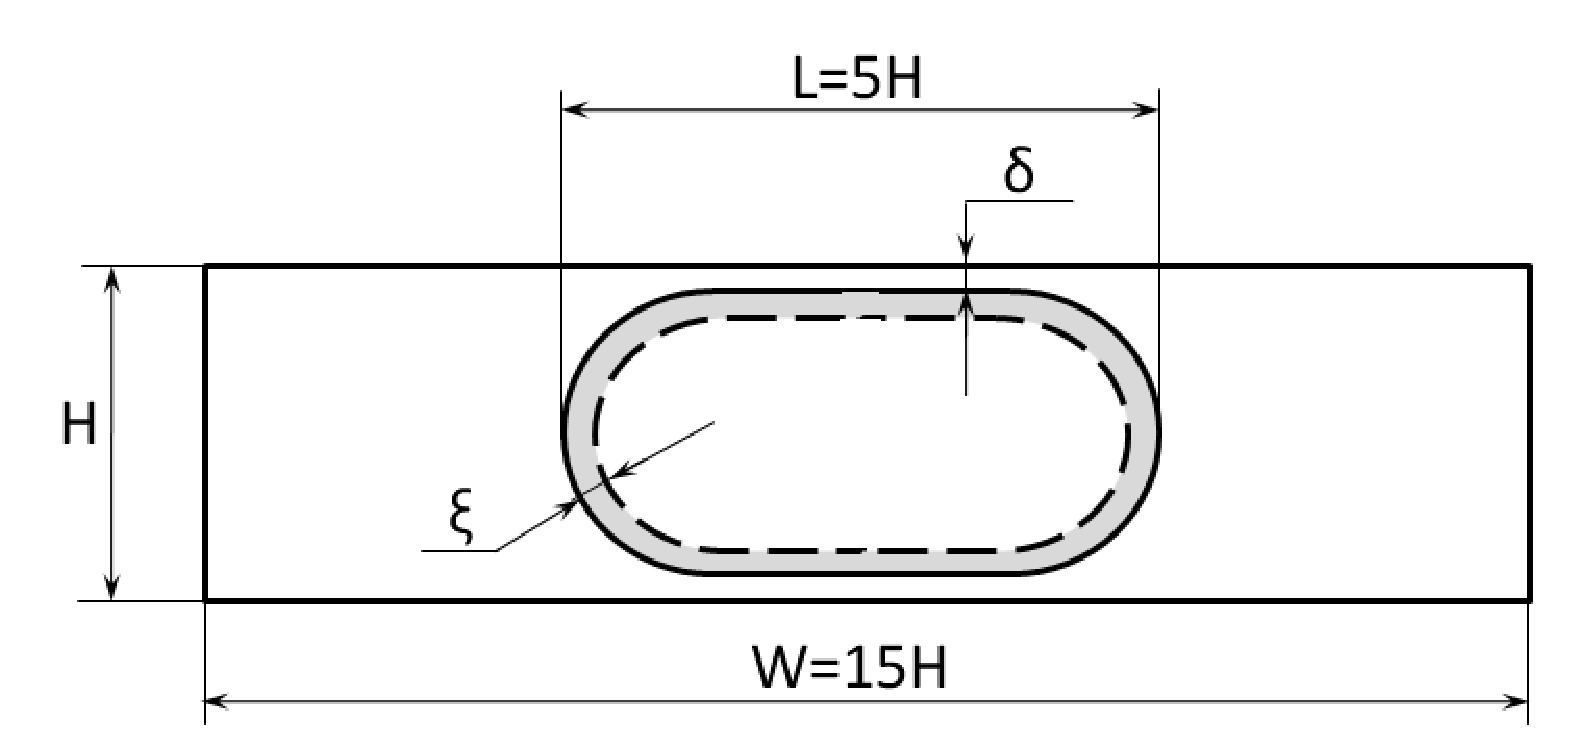
\includegraphics[width=0.97\textwidth]{Figures/benchmark.eps}
\caption{The benchmark sketch. $\delta$ corresponds to film thickness. $\xi$ corresponds to the interface thickness. We take microchannel length to be 15 times larger than height.
\label{fig:benchmark:sketch}}
\end{figure}


\section{Results}
\subsection{The nondimensionalization and initialization procedure}
We now introduce the procedure of nondimensionalization, as well as
the initialization techniques we used to be able to determine parameters necessary for
simulation. The capillary number governs the interface thickness and is defined as:
\begin{equation}
Ca=\frac{U_{\mathrm{bubble}} \mu_{\mathrm{liq}}}{\gamma},
\end{equation}
where $\mu_{\mathrm{liq}}$ is the liquid viscosity, and $\gamma$ is the surface tension. The
bubble velocity $U_{\mathrm{bubble}}$ is taken in the center of the bubble where the film
thickness is examined.
While parameters such as $\mu_{\mathrm{liq}}$, $\gamma$ and the capillary number $\Ca$ are given
or defined through the model parameters, the bubble velocity $U_{\mathrm{bubble}}$ is not given
explicitly.
In the simulation we approximately match and initialize the velocity with the
Poiseuille profile center velocity, which is given by the equation:
\begin{equation}
\begin{aligned}
U_{\mathrm{bubble}} \approx U_{\mathrm{liq}}=\frac{H_{\mathrm{eff}}^2}{8
\mu_{\mathrm{liq}}}\frac{\mathrm{d}P}{\mathrm{d}x}\\
U_{\mathrm{bubble}}\approx
\frac{{(N_y-2)}^2}{\frac{8}{6}(\tau_{\mathrm{liq}}-\frac{1}{2})}\frac{\mathrm{d}P}{\mathrm{d}
x } ,
\end{aligned}
\end{equation}
where $N_y$ is the grid number in the vertical direction. As it will be discussed further, the
effective channel width is defined as $H_{\mathrm{eff}}=N_y-2$ because of bounce-back nodes.
By taking the Poiseuille profile one can estimate the body force through the
capillary number and grid resolution:
\begin{equation}
\label{poiseuille:velocity:center}
\begin{aligned}
&\frac{\mathrm{d}P}{\mathrm{d}x}=\frac{8}{{(N_y-2)}^2}\gamma Ca.
\end{aligned}
\end{equation}
The body force (\ref{poiseuille:velocity:center}) applied to the problem will cause the bubble
velocity different from the implied by the capillary number because of the multiphase flow. That's
why to achieve the 
desired velocity and the
capillary number the iteration procedure to find the appropriate body force needs to be done.
However, the initialization body force given by (\ref{poiseuille:velocity:center}) is a good
starting approximation point. 

After one calculates the parameters necessary to run a simulation, one needs to
initialize the macroscopic fields and particle populations.
The velocity is initialized with $0$ everywhere. Populations are initialized
with the equilibrium values for the binary liquid model, including all the phase
gradients and Laplacians. The liquid phase is initialized with $\phi = 1$ and the
gas phase is initialized with $\phi = -1$. Though the initial film thickness
is not involved in the final result for the front meniscus (see Fig.
\ref{fig:different:initialization:widths}) we keep the initialized film
thickness as close as possible to the already obtained numerical film
thickness values \cite{giavedoni-numerical}. This is done to minimize
the convergence simulation time, as starting far away from the steady-state requies
additional time for the relaxation.
\begin{figure}
\includegraphics*[bb=-15 360 630 430,width=0.97\textwidth]
{Figures/Init/initbegin12.eps}
\includegraphics*[bb=-15 360 630
430,width=0.97\textwidth]{Figures/Init/initfinish12.eps}\\
\includegraphics*[bb=-15 360 630 430,
width=0.97\textwidth]{Figures/Init/initbegin16.eps}
\includegraphics*[bb=-15 360 630
430,width=0.97\textwidth]{Figures/Init/initfinish16.eps}\\
\includegraphics*[bb=-15 360 630 430,
width=0.97\textwidth]{Figures/Init/initbegin20.eps}
\includegraphics*[bb=-15 360 630
430,width=0.97\textwidth]{Figures/Init/initfinish20.eps}\\
\caption{The phase plots for different bubble widths as
$H_{\mathrm{eff}}-12$, $H_{\mathrm{eff}}-16$ and
$H_{\mathrm{eff}}-20$. The grid for the simulation is $102 \times 1501$. The results are rescaled
on $N_y$.The phase
profiles were obtained after $2\cdot10^5$ time steps. One can see that even if the
system is initialized with different bubble volumes, the bubbles always relax
to a shape where the film thickness is conserved. For the given parameters the
interface thickness rescaled at the effective channel width $H_{\mathrm{eff}}$  is
$0.0701$,$0.0697$,$0.0692$ measured at the dimensionless coordinate $x=13$.
\label{fig:different:initialization:widths}}
\end{figure}

Here, two different examples are presented that quantitatively show the
initialization procedure for quite different capillary numbers. In these
examples we use $k=0.04$ and $A=0.04$ as optimal binary liquid model parameters.
That explicitly implies the surface tension to be $\sqrt{\frac{8 k
A}{9}}=0.0377$ and the characteristic length of the interface
$5\sqrt{\frac{k}{A}}=5$ lattice boltzmann units. For the sake of simplicity and
stability the relaxation times for liquid and gas phases are taken as
$\tau_{\mathrm{liq}}=2.5$ and $\tau_{\mathrm{gas}}=0.7$, which corresponds
to a gas-liquid kinematic viscosity ratio of $10$.
\begin{description}
 \item[I \bm{$Ca=0.005$}]
  The film width for such small Capillary numbers \cite{bretherton} is
given by the equation:
  \begin{equation}
  \frac{h_{\infty}}{H_{\mathrm{eff}}}=0.6687 \Ca^{2/3}=0.0194.
  \end{equation}
Thus, the film
thickness occupies around $2$ percent of the whole channel height. Let us impose that $8$ lattice
units are required to resolve  $2$ percent of the channel. Note that $5$ out of $8$ these lattice
units
($62.5$ percent) are used to resolve the phase interface. Therefore the channel width is $400$
lattice units.

We take the bubble length as $5$ channel widths
  and the distance between bubbles is $2$ bubble lengths. This gives a
grid size of $400 \times 6000$. In terms of computer memory
requirements, the calculations with double precision accuracy demand:
\begin{equation}
\begin{aligned}
&2\text{ sets of populations } \times \,\, 8\,\, \text{bytes per population
} \times \,\, 9 \text{ number of
populations}\\
&\times\,400\,\times\,6000\approx 345 \mathrm{MB}. 
\end{aligned}
\end{equation}
Even with this naive assumption for the $62.5$ percent resolution of the interface width of the film
width, one can get the memory
requirement of $345 \mathrm{MB}$. 

After resolving the interface one can  calculate the
  velocity from the capillary number as:
  \begin{equation}
  U_{\mathrm{bubble}}=0.005 \frac{\gamma}{\mu_{\mathrm{slug}}}=0.005
\frac{0.0377}{0.6666}=2.82 \cdot10^{-4},
  \end{equation}
  where $\mu_{\mathrm{slug}}=1/3 (2.5-0.5)=0.6666$.
  This velocity implies the following pressure gradient calculated from the
  Poiseuille flow solution, Eq. \ref{poiseuille:velocity:center}: 
  \begin{equation}
  \begin{aligned}
  \frac{\mathrm{d}P}{\mathrm{d}x}=9.42 \cdot 10^{-9}.
  \end{aligned}
  \end{equation}
Note the velocity is directly
involved in calculation of the physical time step. Small velocites imply longer running simulations:
\begin{equation}
\Delta t =\frac{U_{\mathrm{LBM}}}{U_{\mathrm{phys}}} \Delta x ,
\end{equation}
where for example the real velocities in the physical world can reach
approximately $1$ m/s and physical channel height up to $1$ mm. In this case one
can easily approximate the physical time step during one lattice Boltzmann iteration:
\begin{equation}
\Delta t = 7.05 \cdot 10^{-10} \,\mathrm{s}
\end{equation}
which is small. A typical simulation runs approximately
$100000-300000$ time steps due to computational resources. That gives 
physical time simulation around $10^{-5}-10^{-4}\,\mathrm{s}$, which is
probably not enough for physical system to come to the pseudo steady state.

 \item[II $\bm{Ca=0.05}$] 
   The parameters in the previous subsection imply long
simulations for system to come to equilibrium and this number increase with decrease of the
capillary number. Bretherton obtained the analytical solution for the range of low capillary numbers
less than
  $0.005$. However, a lot of simulations extended it to the range of Capillary numbers greater than
$0.005$, and to higher Reynolds numbers. One can refer to figures
  \ref{fig:giavedoni:planar} and \ref{fig:heil:planar} taken from the work of
  \citet{giavedoni-numerical,heil-bretherton}, who crossvalidated their
  simulations with Bretherton and each other. Even though the LBM can simulate
flows with small capillary numbers, i.e. less than $0.005$, the simulation time
is relatively long. Therefore, we focus our work on the simulations of
\citet{giavedoni-numerical} who crossvalidated
results for all ranges of capillary numbers.  Our intention is
  to show proper physics behavior for moderate parameters
which
  can be easily and quickly validated on a computer.
  One can see from Fig. \ref{fig:heil:planar} that the width for the
  Capillary number $0.05$ ranges from $0.12$ to $0.15$, while the Reynolds
  number ranges from $0$ to $300$.

  The film width for such small Capillary numbers is taken from
  \ref{fig:heil:planar}, and for Reynolds number $40$ equals $0.12$. We want to
  resolve $6\%$ of whole channel width with $12$ lattice units, where $5$
lattice units are related to the interface resolution.  Therefore the channel
  width is $200$ lattice units. Therefore using the assumptions for the benchmark 
the grid size is $200 \times 3000$. The velocity can be
calculated from the Capillary number as:
  \begin{equation}
  U_{\mathrm{bubble}}=0.05 \frac{\gamma}{\mu_{\mathrm{liq}}}=0.05 \frac{0.037712}{0.6666}=2.82\cdot
  10^{-3}.
  \end{equation}
  The velocity implies the following pressure gradient calculated from the
  Poiseuille flow solution:
  \begin{equation}
  \begin{aligned}
  &\frac{\mathrm{d}P}{\mathrm{d}x}=\frac{8}{N_y^2}\gamma Ca=3.77\cdot10^{-7}.
  \end{aligned}
  \end{equation}
  Our approach to the initial conditions is  to take values from the previously performed
numerical simulations and to calculate the grid sizes from them, matching the
body force gradient through the solution of Poiseuille flow.

\end{description}
\begin{figure}
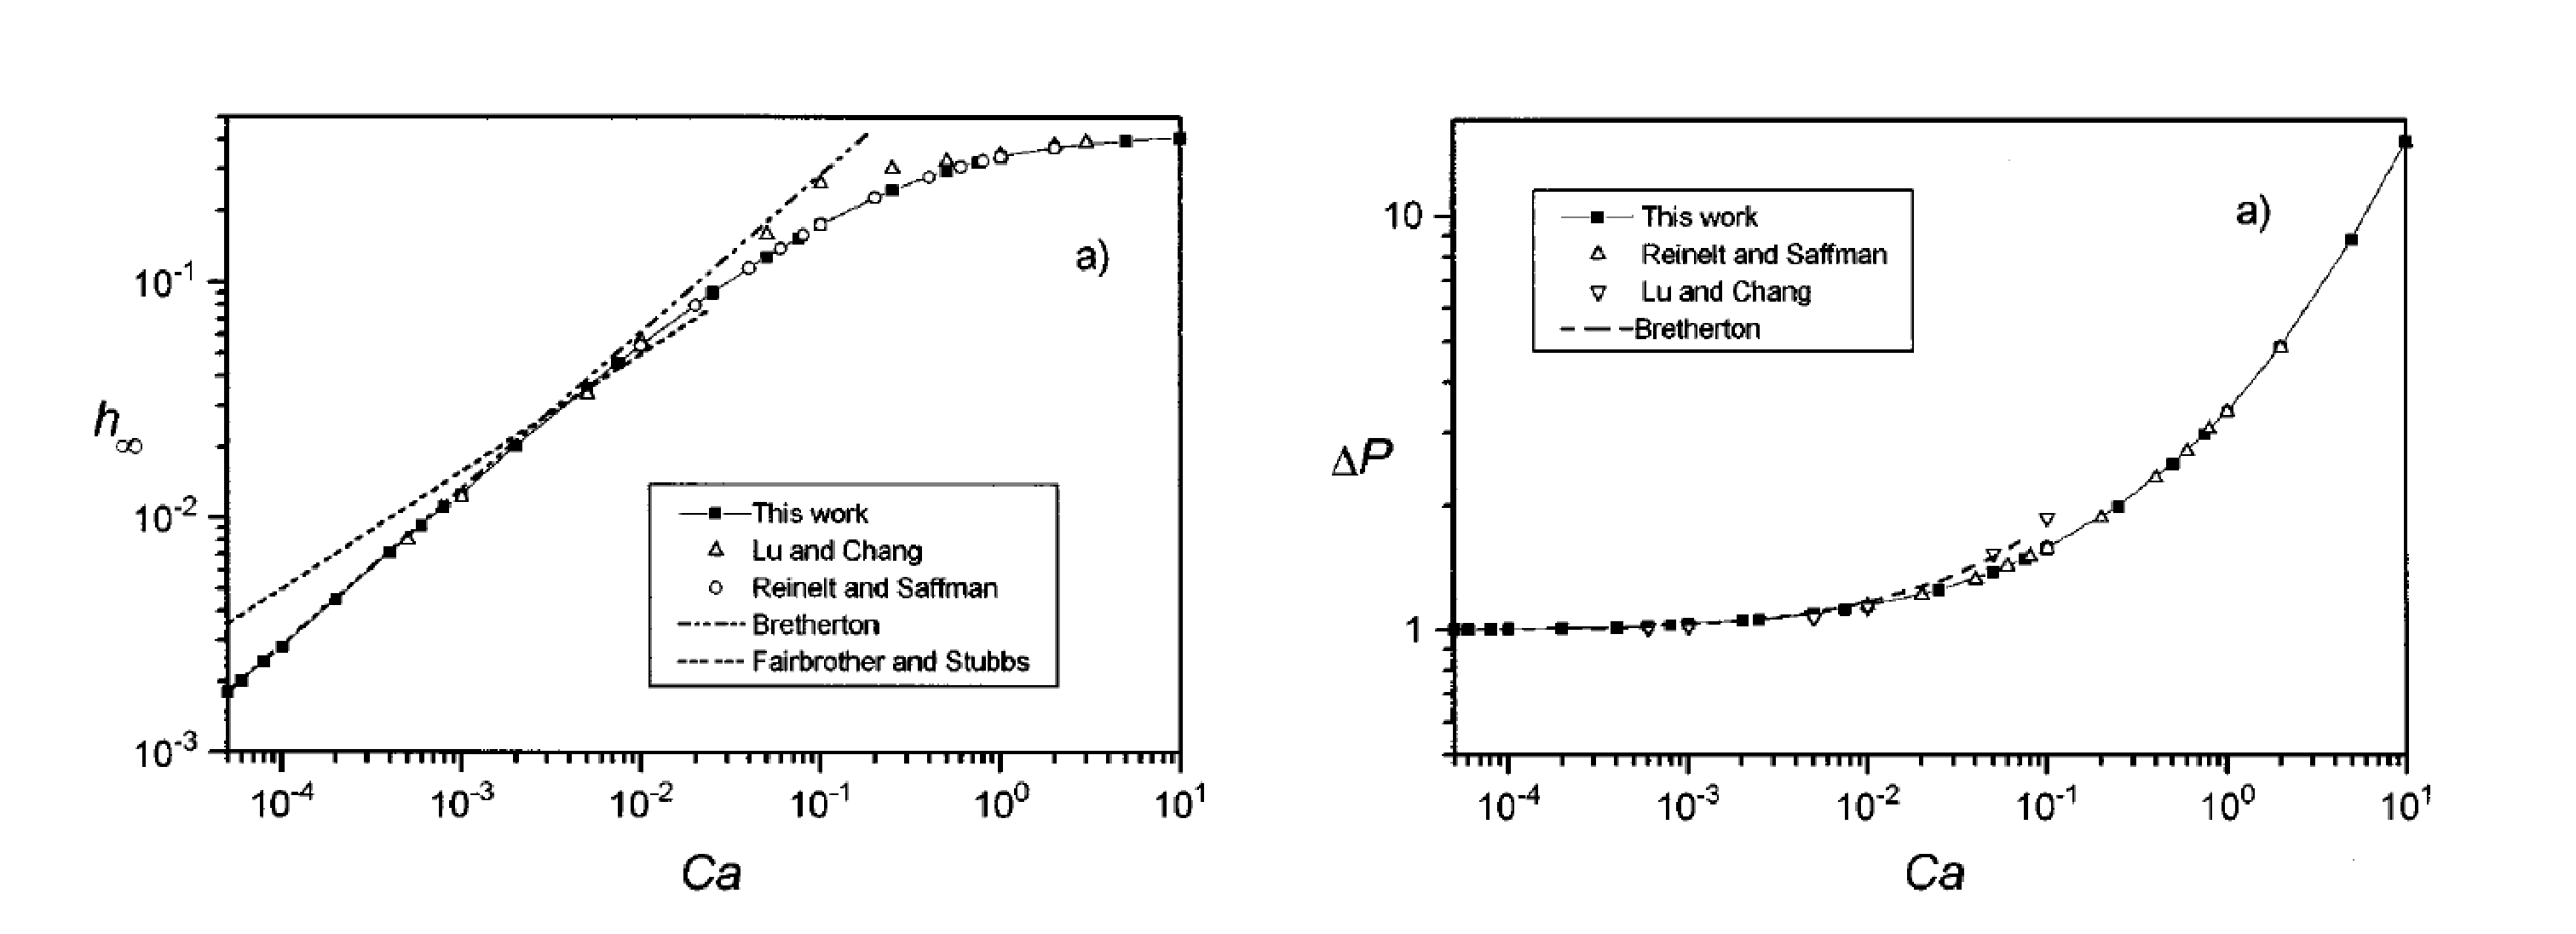
\includegraphics[width=0.97\textwidth]{Figures/giavedoni_planar.eps}
\caption{\citet{giavedoni-numerical} gathered results across the
literature for different Capillary numbers. Note that results are scaled on a half-width of the
channel. \label{fig:giavedoni:planar}}
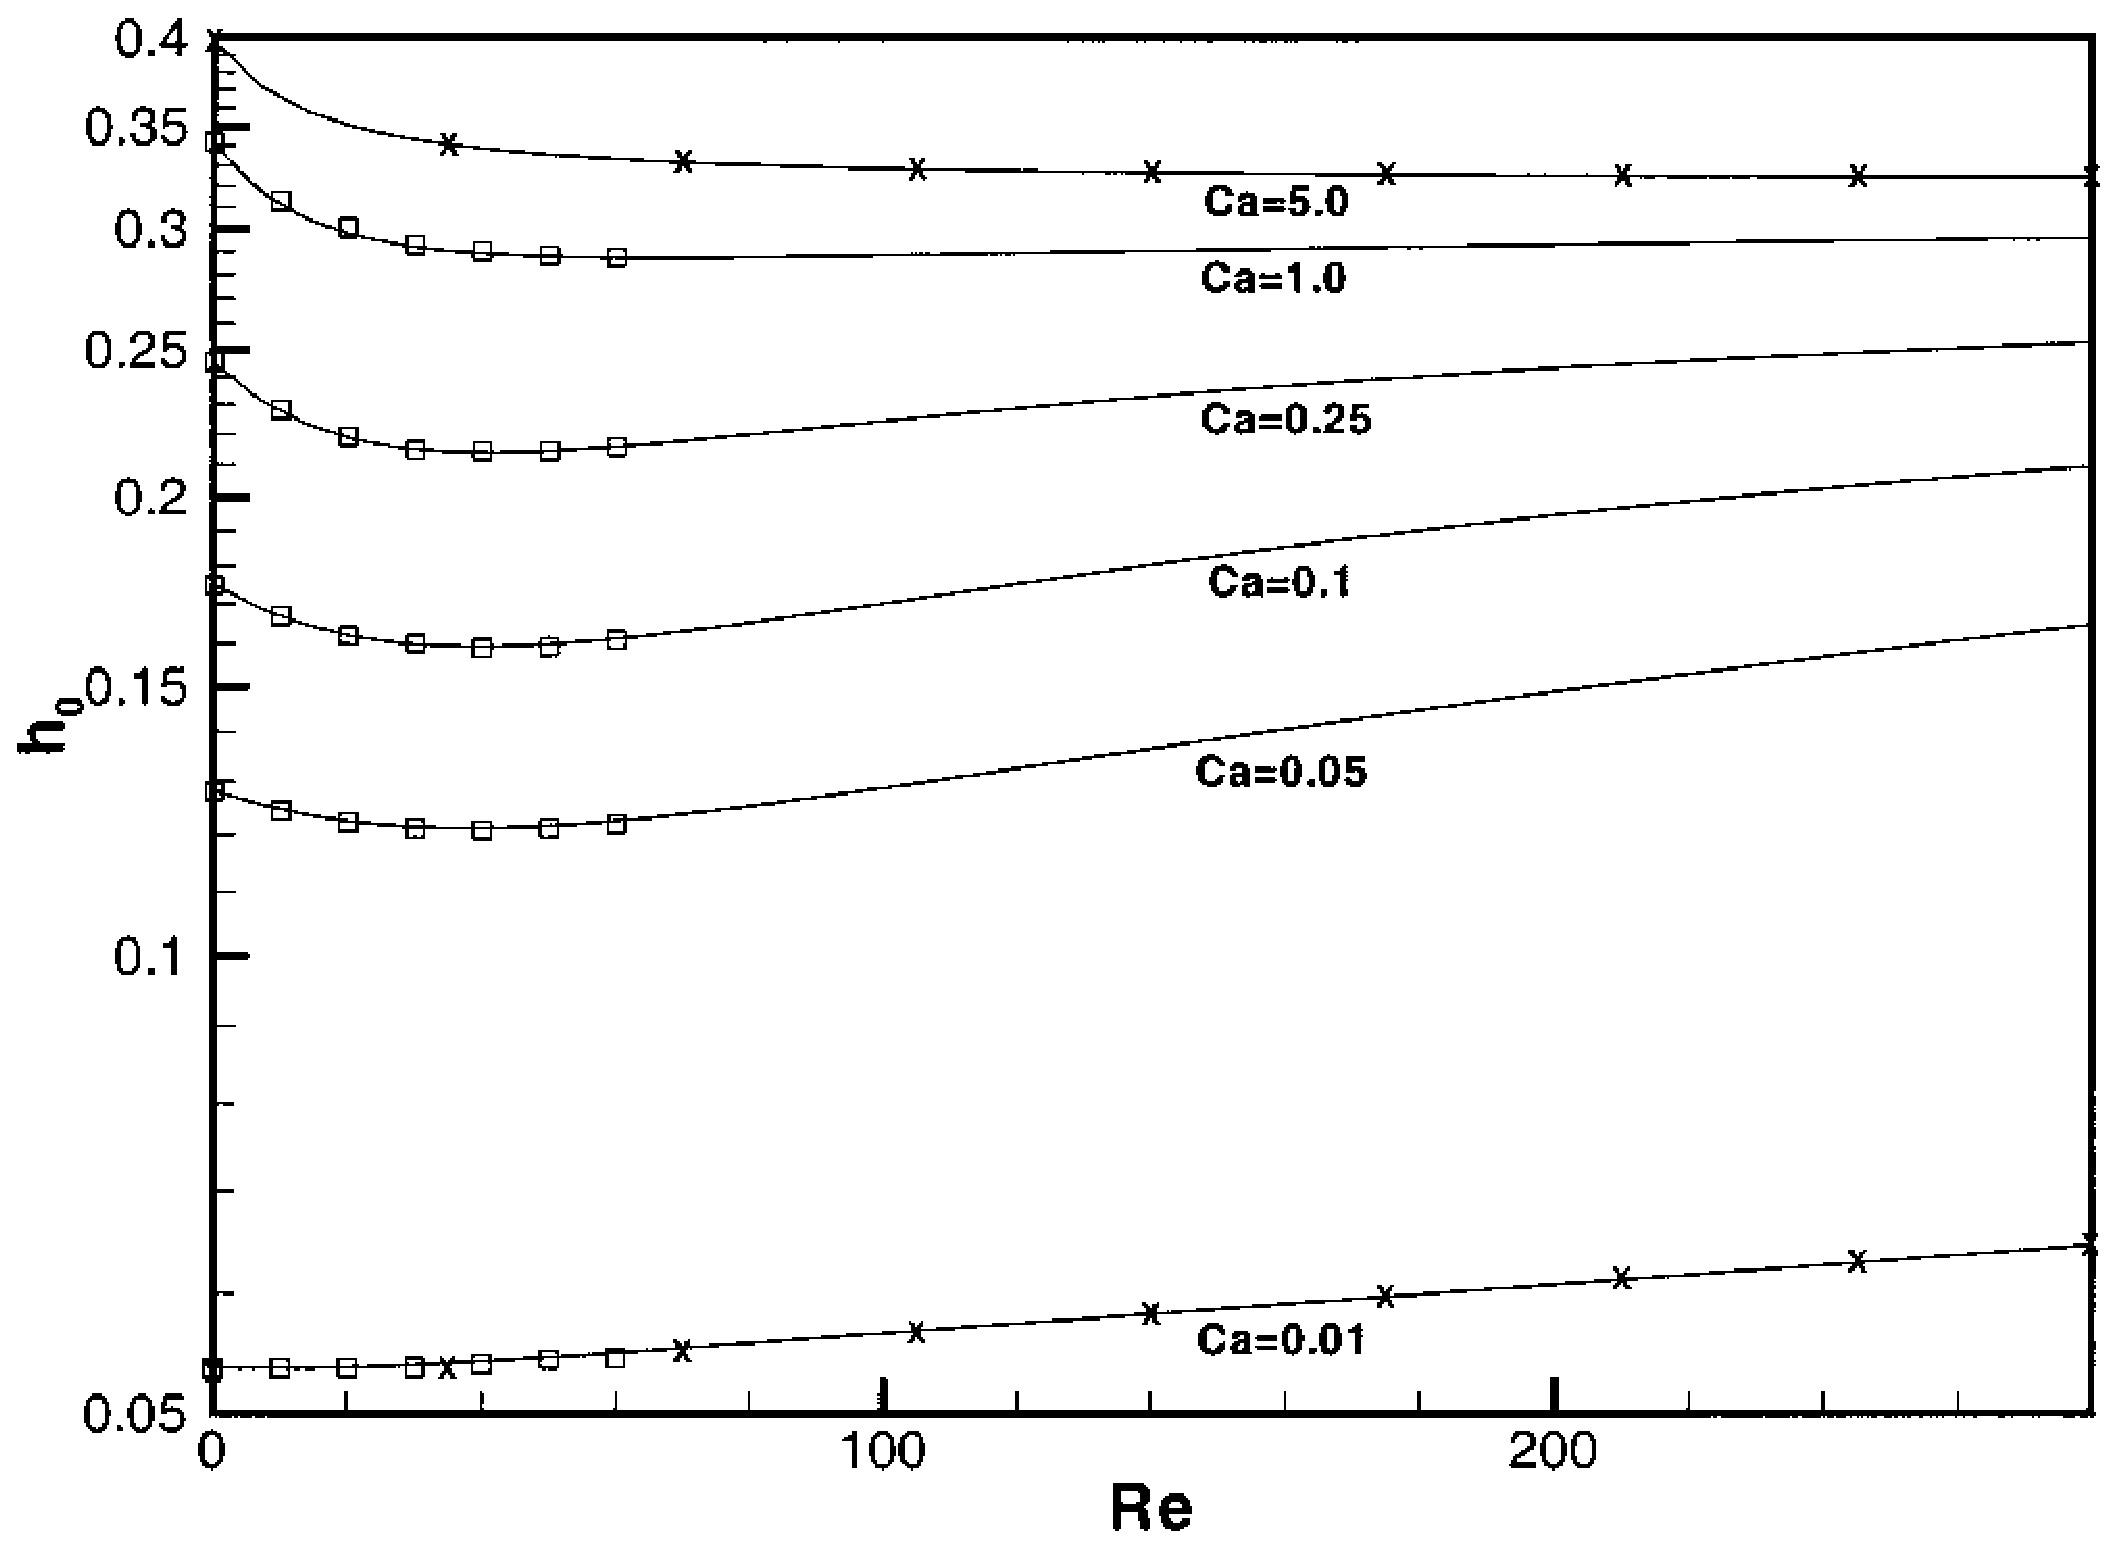
\includegraphics[width=0.97\textwidth]{Figures/heil-planar.eps}
\caption{\citet{heil-bretherton} performed simulations for different ranges of
Capillary numbers and Reynolds numbers. Note that results are scaled on a half-width of the channel.
\label{fig:heil:planar}}
\end{figure}
Note that we base the initialization techniques on correlations for the
capillary number and the body force. However, in the binary liquid framework
those correlations are only approximate. The stronggest assumption lies
in calculating the body force from the Poiseuille velocity profile.
In reality, the less viscous bubble will have a slippage
factor and its velocity is larger than the surrounding liquid velocity. By
substituting the obtained velocity back to the capillary number equation the
larger capillary number can be obtained. While we present the initialization
tips, in practice one needs to take the bubble velocity from the simulations and
recalculate all the necessary characteristics or in other words adjust the
forcing to obtain the desired velocity/capillary number.

\subsection{Grid refinement}
To properly estimate the interface resolution one needs to study the convergence
of the results as a function of the grid resolution. To do that, all parameters are held fixed,
including the bubble velocity, the capillary number, and only the grid
resolution is changed. Our goal is to determine the ratio of the interface width to 
film thickness where results are not dependent on the grid resolution.

We illustrate the procedure for the capillary number
$0.05$. As was pointed out earlier, the film thickness in that case is $6$ percent of the effective
channel $H_{\mathrm{eff}}$.
Note that in the case of the half-way bounce-back walls \cite{yu} which are used in the
simulations one needs to calculate the film thickness as:
\begin{equation}
\delta=(\phi_0-0.5)/(N_y-2),
\end{equation}
where $\phi_0$ is the grid coordinate where phase field is $0$, $N_y-2$
is related to the effective channel height. That can be cleared out by the following explanations.
If the grid number in the vertical direction is $N_y$ then one has $N_y-1$ regions which represent
domain. The effective wall location is in the middle between bounce-back and fluid nodes giving
overall $N_y-2$ representing the channel width. Note that it is a big
simplification to impose the boundary in the middle beetween the bounce-back
node and the fluid node which give rise to the viscosity dependent location of
the wall \cite{ginzburg-multireflection}, however the effective location of the wall for the
multiphase models to the best authors' knowledge is not yet derived. In the case of $\delta=0.06$
the
initial grid size is $N_y=102$, which gives the horizontal grid size as $N_x=15(N_y-2)=1500$.
The bubble is initialized as a rectangular box with coordinates
$y=7\dots N_y-8$, $x=\frac{N_x}{3}\dots \frac{2 N_x}{3}$ and phase
$\phi_{\mathrm{bubble}}=-1$. All other nodes are initialized with the phase field
$\phi=1$. The force gradient can be estimated through the Poiseuille
profile formula, Eq.~\ref{poiseuille:velocity:center}, and it equals
$1.508 \cdot 10^{-6}$ lattice units.

After choosing the reference parameters, the grid refinement procedure
needs to keep the macroscopic parameters constant.  It is easy to check
that it yields the following quantity to
be independent of grid size
$H_{\mathrm{eff}}^2\frac{\mathrm{d}P}{\mathrm{d}x}=(N_y-2)^2\frac{\mathrm{d}P}{\mathrm{d}
x } = \mathrm{const}$. We performed a number of simulations for the prescribed grids. The
simulations in terms of grid numbers $N_x$, $N_y$, the film thickness $\delta$, center bubble
velocity $U_{bubble}$ are summarized in Table \ref{table:parameters:grid:refinement}.
The unified scaled profiles are shown in Fig. \ref{fig:grid:profiles}. One can
see the visual results converge for $H_{\mathrm{eff}}\geq 175$. However, one can see
that with proper initialization techniques, large enough time and the wall
wettability, results are different only in the 3rd digit even for
underresolved film widths. To calculate how well the interface thickness is
resolved, the ratio of the interface thickness to the film width thickness is calculated. The
interface itself occupies approximately $5 \xi$, where
$\xi=\sqrt{k/A}=1$. The ratio of the interface width to the film thickness $5\xi/H_{\mathrm{film}}$
 is shown in Table \ref{table:parameters:grid:refinement}. Based on results one can conclude that
 the interface needs to be resolved as $40-50$ percent of the
expected film width for simulations to be convergent. We further examine the
velocities in the center of the bubble to calculate the Capillary number. One can see from Table
\ref{table:parameters:grid:refinement} that the bubble velocities are pretty consistent and the
calculated capillary number corresponding to those values is $0.07$, which is slightly
larger than the expected capillary number. The corresponding error can be
attributed to the density and viscosity ratios which are much larger in the
Bretherton problem and Poiseuille profile body force initialization.
\begin{figure}
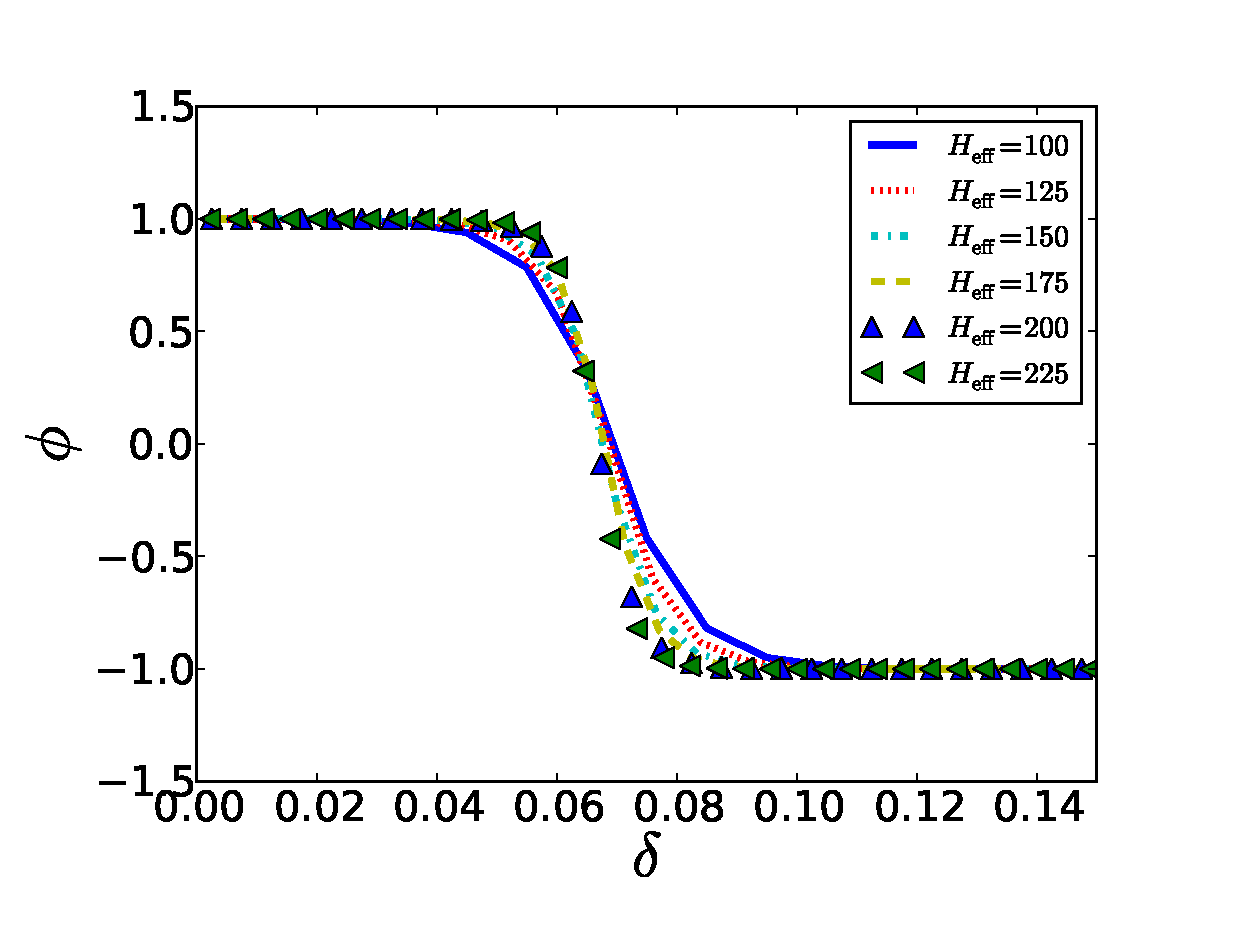
\includegraphics[width=0.97\textwidth]{Figures/Grid/norm_grid_profs.eps}
\caption{Grid-refined profiles for the effective
channel widths
$H_{\mathrm{eff}}=100,125,150,175,200,225$.$\delta$ is scaled on $H_{eff}$ and $\delta=0$
corresponds to the wall location. The profiles were taken at $x=14$ nondimensional coordinate.
Capillary number is $Ca=0.05$. Capillary number obtained from simulations $Ca=0.07$. One can
see
convergent results even for the underresolved film
thickness.\label{fig:grid:profiles}}
\end{figure}
%Here will be a consolidated table
\begin{table}
\begin{tabularx}{0.97\textwidth}{|X|X|X|X|X|X|}
\hline
$N_x$&$N_y$&$\delta$&$U_{bubble}$&$\frac{5\xi}{H_{\mathrm{film}}}$&$N_{iter}$\\
\hline
$1500$&$102$&$0.0694$&$0.0041$&$0.824$&$200000$\\
\hline
$1875$&$127$&$0.0688$&$0.0041$&$0.646$&$250000$\\
\hline
$2250$&$152$&$0.0676$&$0.0040$&$0.539$&$300000$\\
\hline
$2625$&$177$&$0.0679$&$0.0040$&$0.453$&$350000$\\
\hline
$3000$&$202$&$0.0668$&$0.0041$&$0.400$&$400000$\\
\hline
$3375$&$227$&$0.0663$&$0.0039$&$0.355$&$450000$\\
\hline
\end{tabularx}
\caption{The parameters and results for studying grid resolution simulations. Domain simulated is
of size $N_x\, \mathrm{x}\, N_y$. $U_{bubble}$ is center
bubble velocity measured at the scaled to $H_eff$ $x=14.0$.
$5\xi$ is the interface thickness. $H_{\mathrm{film}}=\delta (N_y-2)$ is the size of the film in
lattice Boltzmann units. $Ca=0.05$ was taken to initialize the simulation.
\label{table:parameters:grid:refinement}}
\end{table}

\subsection{The influence of the wall gradient}
The simulation results should not depend on the wall wettability. Wettability is defined
through the phase gradient \cite{pooley-contact}, $\partial_n \phi$.  We took a large
enough grid resolution in order for simulations to be consistent -- the grid size was
$177 \times 2626$ and the initial film width was
$12$ lattice boltzmann units, which corresponds to the predicted film thickness.
We examined $11$ different values for the wall
gradient ranging from $-1$ to $1$. The parameters are summarized in Table
\ref{table:parameters:wall:gradient}. The results are consistent among all the
wall gradients given that the interface is resolved in the right way. For 
given wall gradients the values of interface thickness values are of $0.2\%$ relative accuracy.  For
the wall gradients $0.8$
and $1.0$ the
simulations are unstable. One can see the simulated profiles in Fig.
\ref{fig:gradients:profiles}. The latter shows that the negative wall gradient values cause 
unphysical phase values more than $1.0$ near the wall. One should attribute them to the numerical
imposement of wall gradients. Therefore, they do not spoil numerical scheme as whole. Note that
negative values of the phase gradient are
preferable, since the phase of the liquid adjacent to the wall has the value of $1$.
The phase values near the wall are above $1$ and do not interact
with the bubble which has phase value $-1$.  In case of positive
gradients the values near the wall are below $1$, and the gradient profile can
fuse with the values of the gas phase. This case is attributed when to the slug flow when gas
touches the wall.
\begin{figure}
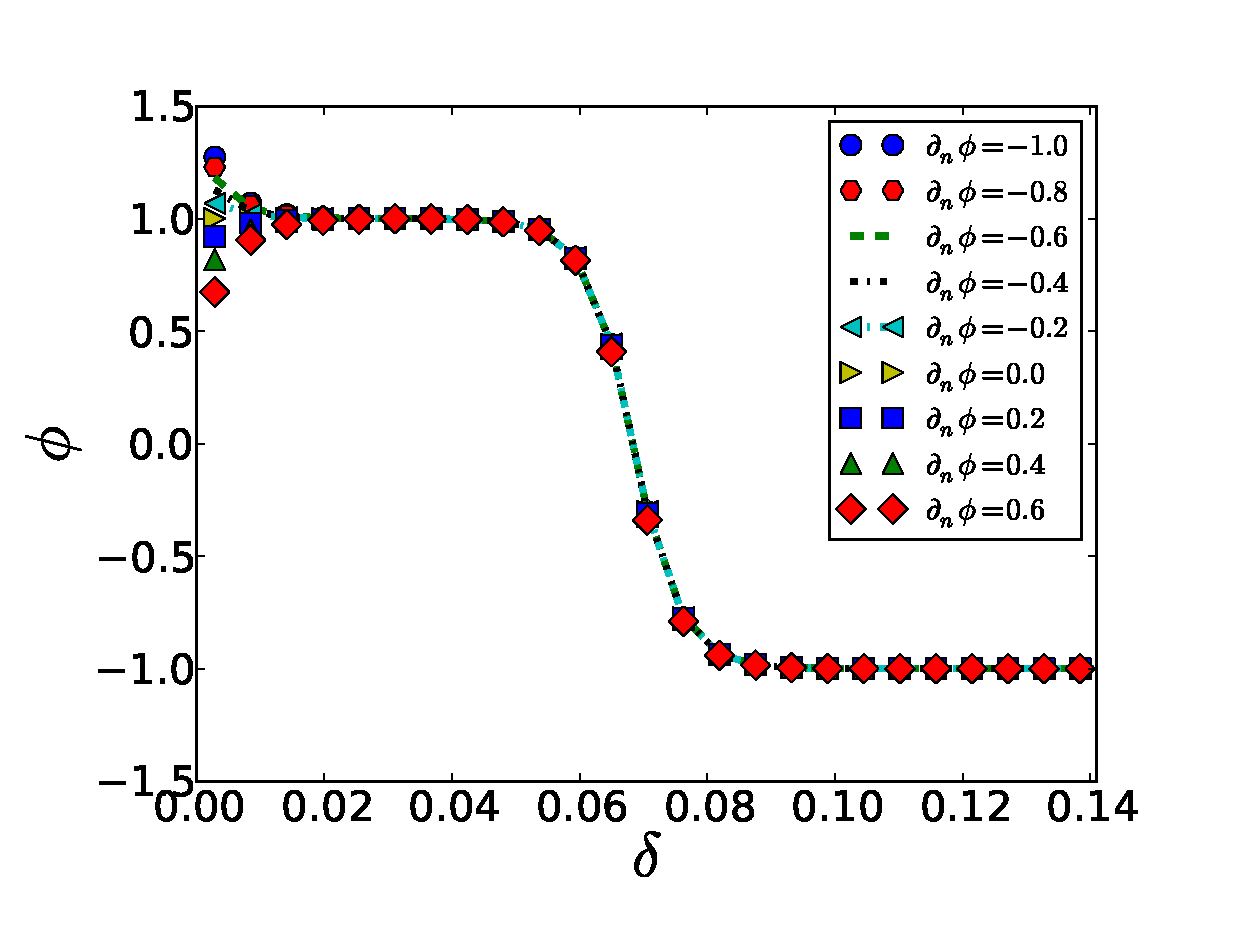
\includegraphics[width=0.97\textwidth]{Figures/Wall/phase_grad_profiles.eps}
\caption{Phase profiles for different wall gradients. One can see that if the width
is properly resolved then the wettability of the wall does affect the film thickness. The
simulations were conducted for $200,000$ iterations. The measured profile was taken at the
nondimensional coordinate scaled to $H_{\mathrm{eff}}$ as $x=11.42$. $Ca=0.05$ was taken to
initialize simulation.
\label{fig:gradients:profiles}
}
\end{figure}

Another question which arises is the influence of the wall gradient on the bubble velocity and the
corresponding capillary number. The shear stress controlled by the wall phase gradient changes the
effective viscosity near the wall, thus changing the bubble velocity as well. If viscosity ratio is
high enough then the free surface motion of the bubble should not be dependent on the shear stress
near the wall.
One can see that if the film thickness is resolved properly the influence of the wall gradient can
be neglected. The center bubble velocities are presented in Table
\ref{table:parameters:wall:gradient}. 
%Fig. \ref{fig:velocities:wall:gradient} shows the center bubble velocity for different
%gradients. 
The average relative error around the mean velocity is $0.1\%$.
% Uncomment if you need this picture
% \begin{figure}
% 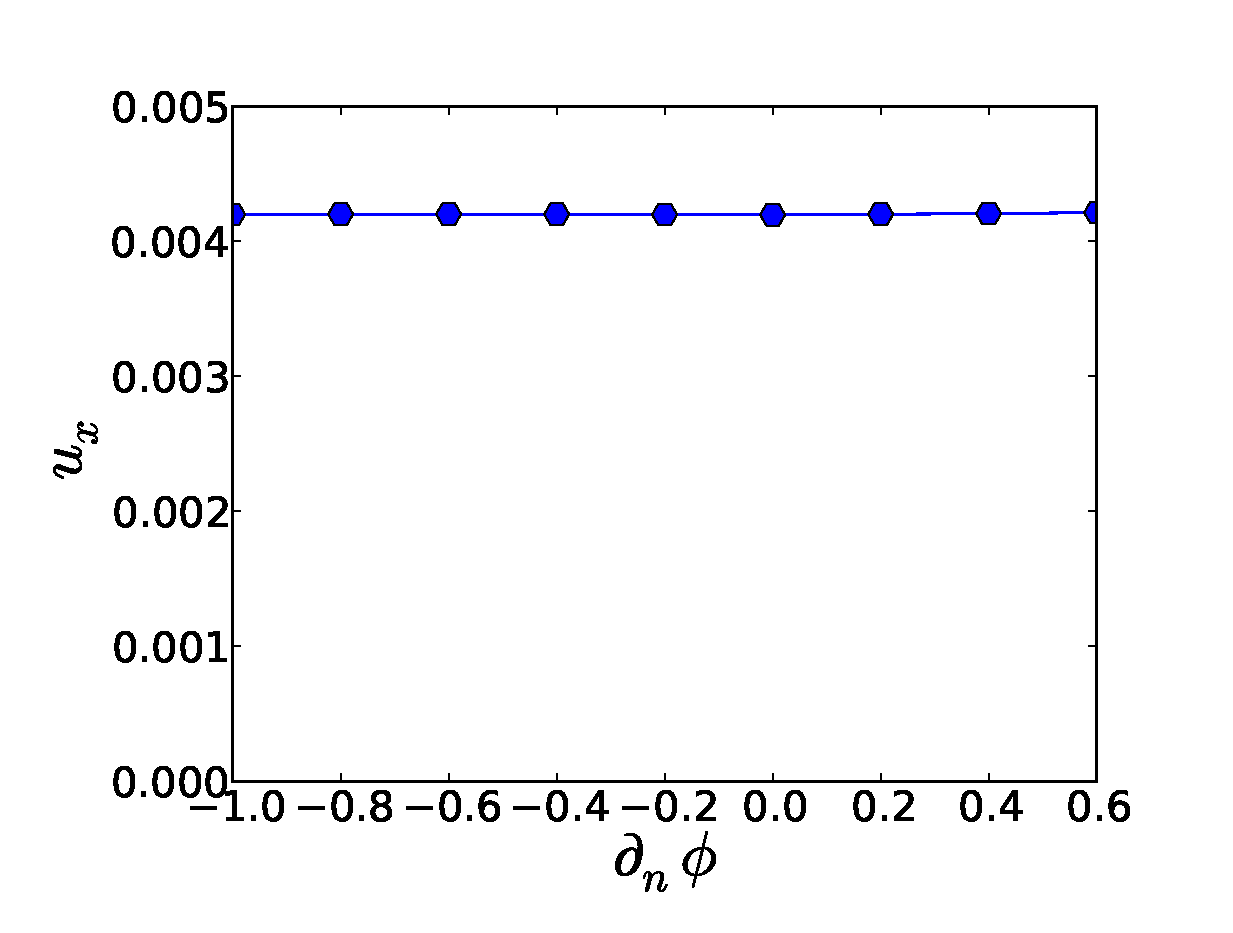
\includegraphics[width=0.97\textwidth]{Figures/Wall/velocities_grad_profiles.eps}
% \caption{The center bubble velocity versus the phase gradient. One can neglect the influence of
% the wall once the film is properly resolved.
% \label{fig:velocities:wall:gradient}
% }
% \end{figure}
\begin{table}
\begin{tabularx}{\textwidth}{|X|X X X X X X X X X X X|}
\hline
$\scriptstyle \partial_n \phi$& $\scriptstyle -1.0$& $\scriptstyle -0.8$&
$\scriptstyle -0.6$&$\scriptstyle -0.4$&$\scriptstyle -0.2$&$\scriptstyle
0.0$&$\scriptstyle 0.2$&$\scriptstyle 0.4$&$\scriptstyle 0.6$&$\scriptstyle 0.8$&$\scriptstyle
1.0$\\
\hline
$\scriptstyle \delta$& $\scriptstyle 0.0633$& $\scriptstyle 0.0634$& $\scriptstyle 0.0634$&
$\scriptstyle 0.0634$& $\scriptstyle 0.0634$& $\scriptstyle 0.0634$& $\scriptstyle 0.0633$&
$\scriptstyle 0.0632$& $\scriptstyle 0.0631$ &$\scriptstyle \mathrm{N/A}$&$\scriptstyle
\mathrm{N/A}$\\
\hline
$\scriptstyle U_{b}$ &$\scriptstyle 0.0041$& $\scriptstyle 0.0042$& $\scriptstyle 0.0042$
&$\scriptstyle 0.0042$ & $\scriptstyle 0.0041$& $\scriptstyle 0.0041$ & $\scriptstyle 0.0042$ &
$\scriptstyle 0.0042$ & $\scriptstyle 0.0042$ & $\scriptstyle \mathrm{N/A}$ &$\scriptstyle
\mathrm{N/A}$\\
\hline
\end{tabularx}
\caption{The parameters and results for studying wall gradient simulations. $U_{b}$ stands for the
center bubble velocity. $\delta$ is the interface thickness. $\partial_n \phi$ is the phase
gradient near the wall responsible for hydrophilic and hydrophobic behavior. The results are
calculated at nondimensional $x=11.42$ after $200000$ time iterations. $Ca=0.05$ was taken to
initialize simulation.
\label{table:parameters:wall:gradient}}
\end{table}

\subsection{Capillary number region}
The purpose of this section is to validate the correlations of
\citet{giavedoni-numerical}, Fig. \ref{fig:giavedoni:planar}, and
\citet{heil-bretherton}, Fig. \ref{fig:heil:planar}, for a range of capillary
numbers. Because of limited computational resources, we skip the
small capillary numbers and compare the film thickness over the capillary number
range from $0.03$ to $0.8$, which is a computationally reasonable task.  
To perform numerical simulations we refer
to the grid refinement section where we established that the interface width should be
at most $50$ percent of the interface width.  We therefore choose the grid to be
$202 \times 3001$. $5$ lattice Boltzmann units do not occupy more than $60$
percent of the effective width. Because the simulation get unstable with
smaller grids and larger gradients, all the capillary number simulations were
performed on the chosen grid. To properly initialize the force gradient, the
proportionality law was utilized. The forcing
$6 \cdot 10^{-6}/16$ was chosen to obtain the predicted capillary
number $0.05$. The forcing for other grids can be obtained using
simple correlations:
\begin{equation}
\begin{aligned}
&Ca_{\mathrm{lit}} \propto U_{\mathrm{bubble}}\\
&U_{\mathrm{bubble}} \propto \frac{\mathrm{d}P}{\mathrm{d}x} N_y^2\\
&Ca_{\mathrm{lit}} \propto \frac{\mathrm{d}P}{\mathrm{d} x} N_y^2 \text{ or }\\
&\frac{\mathrm{d}P}{\mathrm{d} x} \propto \frac{\Ca_{\mathrm{lit}}}{N_y^2},
\end{aligned}
\end{equation}
where the subscript ,,lit'' stands for the predicted capillary number
\cite{giavedoni-numerical,heil-bretherton}. The grid number $N_y$ is not
involved because all simulations are conducted on the same grid.
The pressure gradient can be obtained through the capillary numbers
ratio:
\begin{equation}
\frac{\mathrm{d}P}{\mathrm{d} x}=6 \cdot 10^{-6}/16 \frac{Ca_{\mathrm{lit}}}{0.05}
\end{equation}
The film width is initialized through the capillary numbers ratio as well:
\begin{equation*}
w=12 \frac{Ca_{\mathrm{lit}}}{0.05}
\end{equation*}
The results were obtained after $2\cdot10^5$ steps. Simulation results are presented in Table
\ref{table:parameters:capillary:number}. One can see that the calculated
capillary numbers are overpredicted but the obtained widths are overpredicted
as well due to the improper body force imposement, because of the Poiseuille flow assumption. If one
needs to obtain the desired capillary number, the shooting method for the forcing is
necessary starting as the Poiseuille pressure gradient force as the initial condition. We extracted
results of 
\citet{giavedoni-numerical} and \citet{heil-bretherton} and compared them with our results, shown
in Fig. \ref{fig:capillary:comparison}.
\begin{figure}
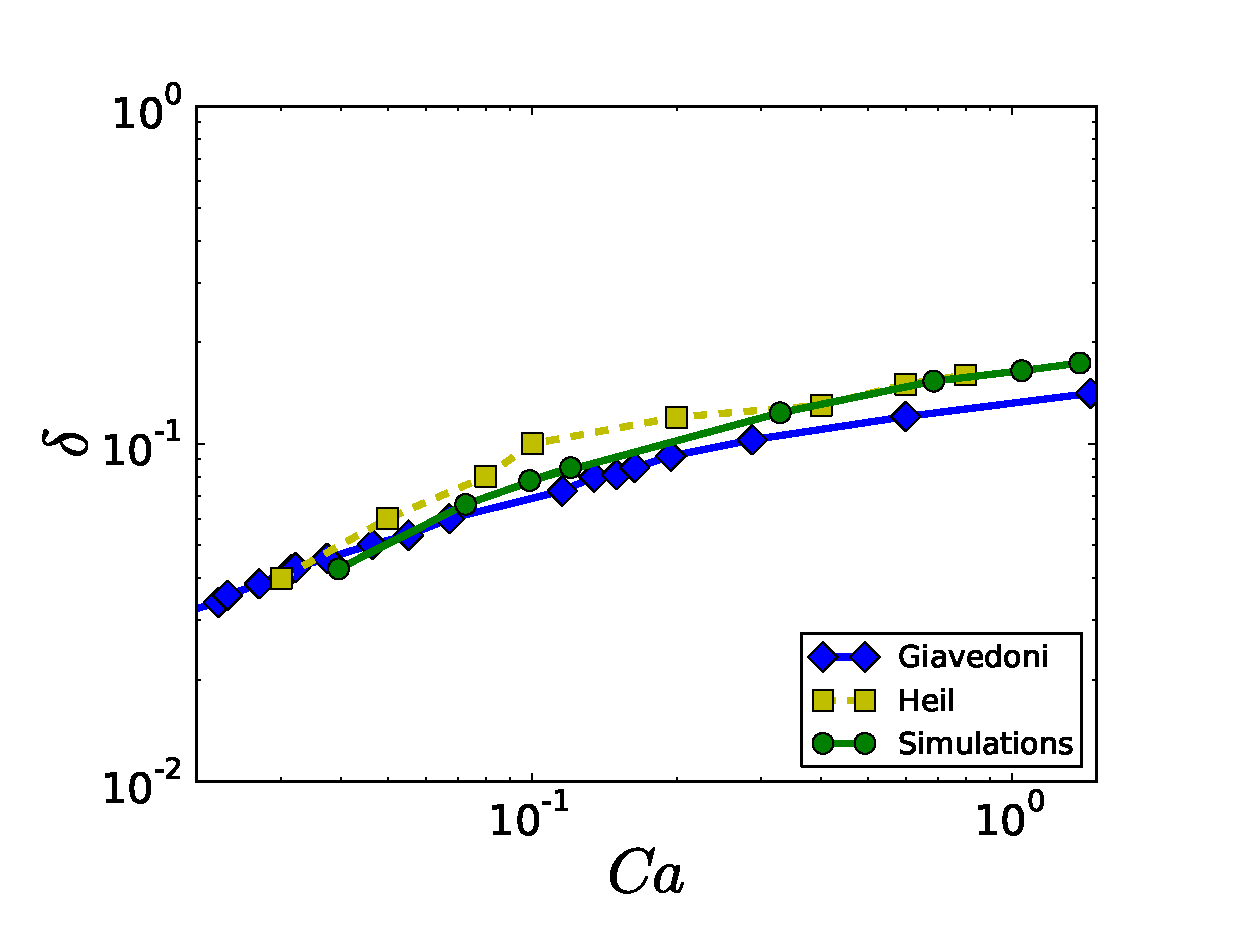
\includegraphics[width=0.97\textwidth]{Figures/Capillary/capillaries_comparison.eps}
\caption{A comparison between simulation results and results of
\citet{giavedoni-numerical} and \citet{heil-bretherton}. One can see a
reasonable agreement. The plots depict the film thickness as a function of the
the capillary number.\label{fig:capillary:comparison}}
\end{figure}

\begin{table}
\begin{tabularx}{\textwidth}{|X|X|X|X|X|X|}
\hline
$Ca_{\mathrm{lit}}$&$\delta_{\mathrm{lit}}$&$x$&$\delta$&$U_b$&$Ca$\\
\hline
$0.03$&$0.04$&$10.0$&$0.042$&$0.0022$&$0.039$\\
\hline
$0.05$&$0.06$&$11.0$&$0.066$&$0.0041$&$0.072$\\
\hline
$0.08$&$0.08$&$13.0$&$0.085$&$0.0068$&$0.120$\\
\hline
$0.1$&$0.1$&$12.5$&$0.077$&$0.0055$&$0.098$\\
\hline
$0.2$&$0.12$&$5.5$&$0.123$&$0.0185$&$0.328$\\
\hline
$0.4$&$0.13$&$4.7$&$0.153$&$0.0388$&$0.686$\\
\hline
$0.6$&$0.15$&$3.0$&$0.164$&$0.0592$&$1.046$\\
\hline
$0.8$&$0.16$&$1.7$&$0.173$&$0.0782$&$1.383$\\
\hline
\end{tabularx}
\caption{The parameters and results for studying capillary number region simulations.
$\delta_{\mathrm{lit}}$ is the film thickness with corresponding $Ca_{\mathrm{lit}}$ taken from
literature. $\delta_{sim}$ is the simulation film thickness with corresponding $Ca$. $U_b$ is the
center bubble velocity taken at location $x$. $Ca$ is based on the measured center bubble velocity
$U_{b}$.
\label{table:parameters:capillary:number}}
\end{table}



\subsection{The film variation over the bubble}

Next, we investigated the qualitative variation of the film thickness over the bubble length.
Though there are simulations for the bubble length for the two-dimensional case, due to
the presentation of data it is hard to extract numerical values from the plots. One can see bubble lengths
variations for the two-dimensional simulations for the range of capillary numbers in Fig.
\ref{fig:sehgal:bubble:length}.
\begin{figure}
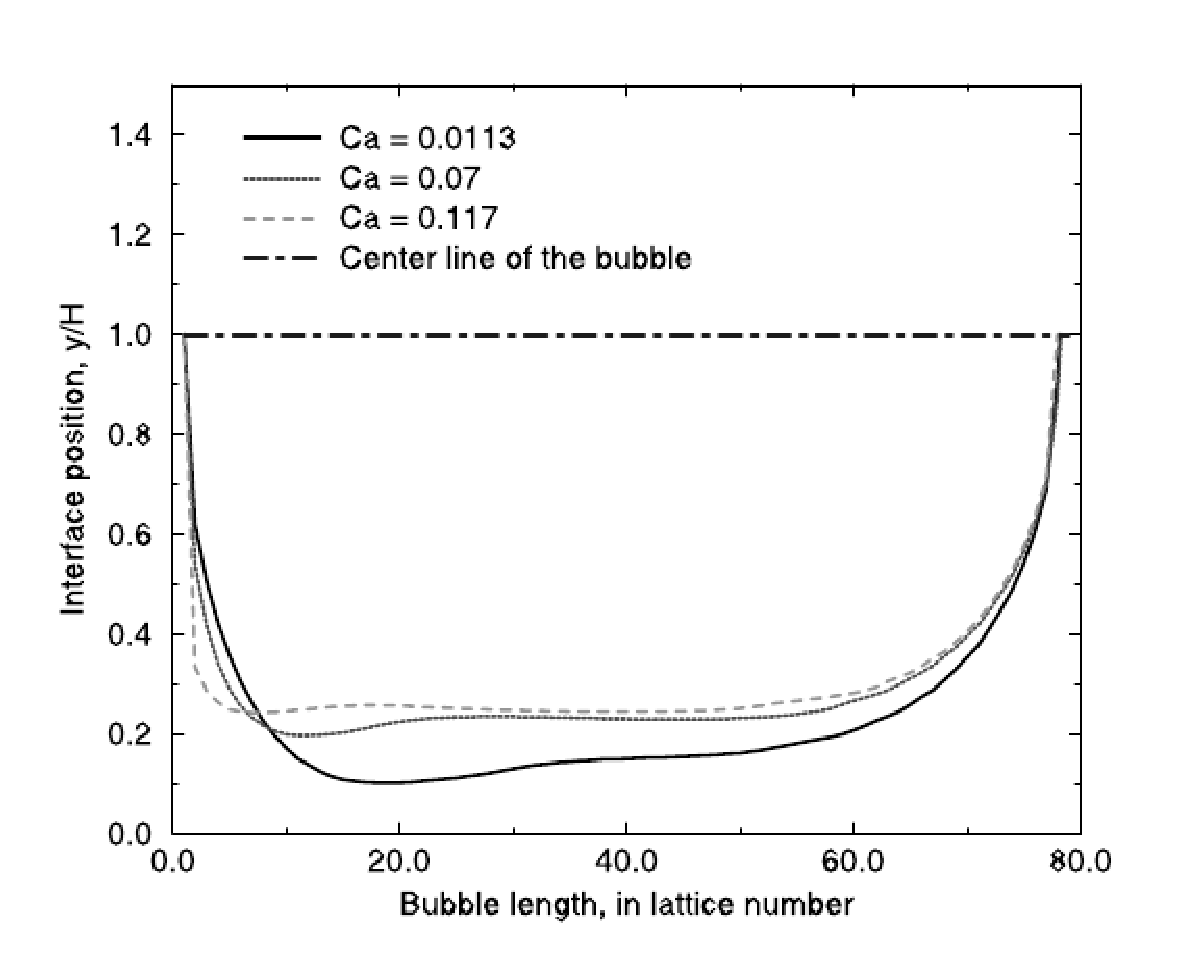
\includegraphics[width=0.47\textwidth]{Figures/Bubble/bubble_sehgal.eps}\hfill
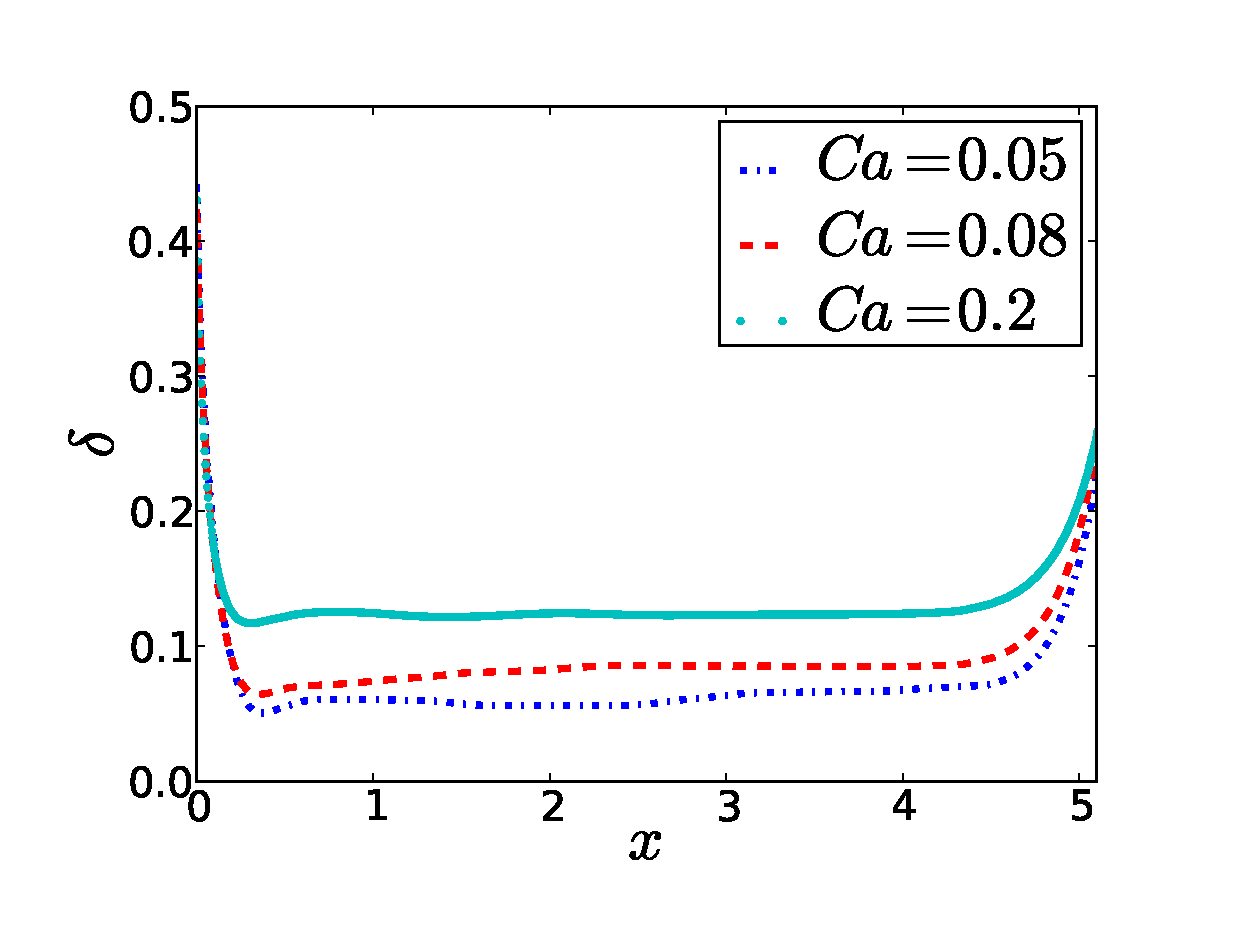
\includegraphics[width=0.47\textwidth]{Figures/Bubble/bubble_length.eps}\\
\caption{The qualitative comparison for the film thickness across
the bubble length. Left (courtesy of \citet{sehgal-microchannel}),
right (present simulations). $x$ is scaled to $H_{\mathrm{eff}}$
and is taken in the flow direction.\label{fig:sehgal:bubble:length}}
\end{figure}
One can see a qualitative agreement, i.e. the thickness increases towards the front meniscus and
rapidly decreases towards the rear meniscus. This shape sometimes is referred as a "bullet" shape.

\subsection{The influence of different viscosities}
The results obtained earlier are taken for the liquid viscosity ratio $10$.
We performed the same simulations for the liquid viscosity ratio of $20$.
The relaxation parameters were taken as $\tau_{\mathrm{liquid}}=4.5$ and $\tau_{\mathrm{bubble}}=0.7$. We
did not find any significant differences with the results obtained earlier. The
comparison for the liquid thicknesses is presented in Fig.
\ref{fig:capillary:viscous}. The results validate our assumption that in
the low capillary flow regime the density ratio does not affect the film thickness,
and that the gas-liquid viscosity ratio of the order $10$ is enough to obtain results
consistent with the Bretherton/Taylor problem.
\begin{figure}
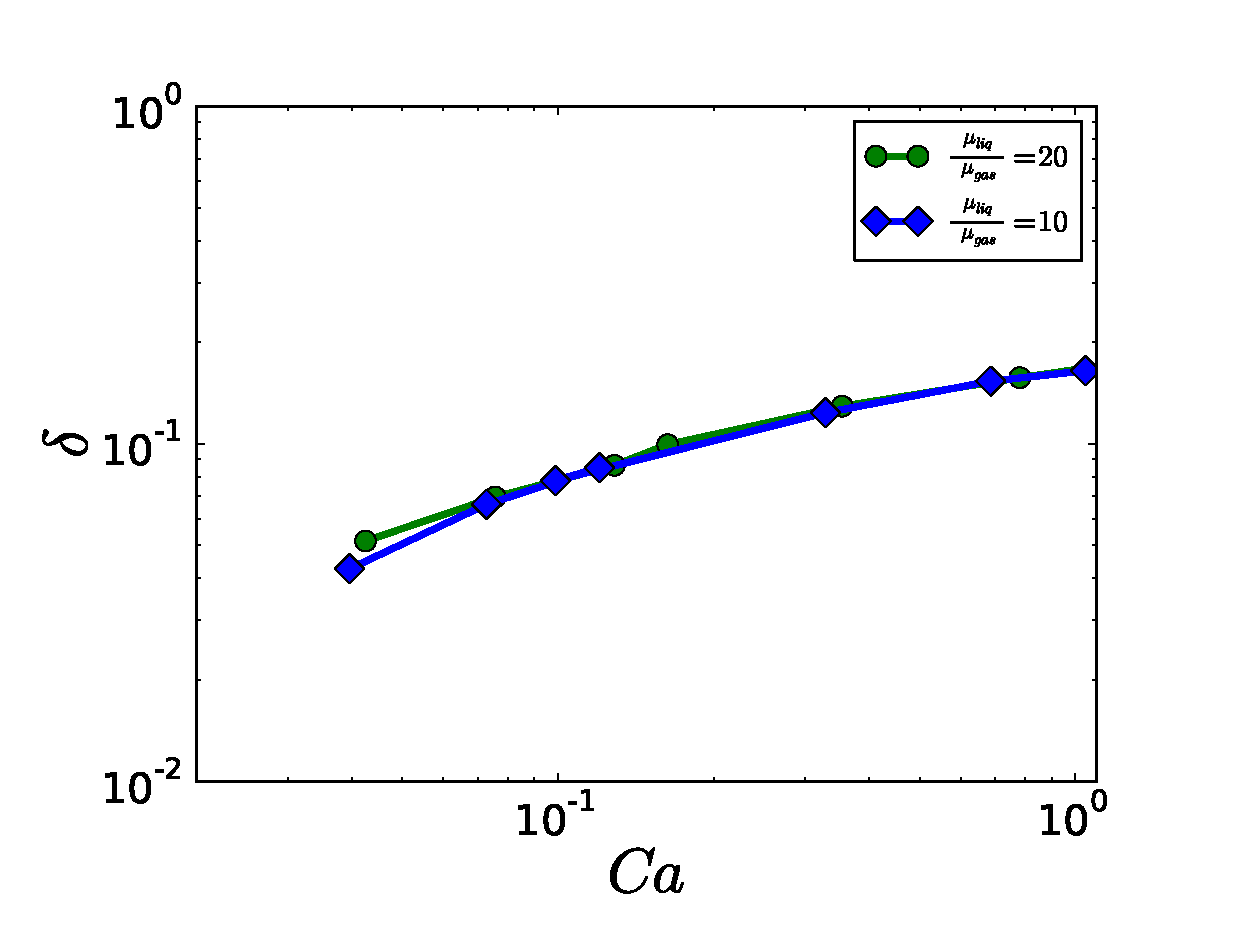
\includegraphics[width=0.97\textwidth]{Figures/Capillary_Viscous/capillaries_viscous.eps}
\caption{The film widths versus capillary number for
$\frac{\mu_{\mathrm{liq}}}{\mu_{\mathrm{gas}}}=10$ and $\frac{\mu_{\mathrm{liq}}}{\mu_{\mathrm{gas}}}=20$. The
results show good consistency and mutual agreement.\label{fig:capillary:viscous}}
\end{figure}

\section{Conclusion}
This work presents numerical tips and a benchmark for the
Bretherton/Taylor problem using the binary liquid lattice Botlzmann method. To obtain correlations
we specifically designed the benchmark. The bubble was chosen long enough for the film thickness to
stabilize. Also, we used periodic boundary conditions for scheme robustness. Thus, the bubble
train was simulated instead of one bubble motion. To avoid the influence of other bubbles
distance between bubbles were chosen as $3$ bubble sizes. The
results show consistency with the previously published numerical results obtained
using other methods in terms of capillary number region, shape of the bubble. It comes with surprise
but with large enough viscosities ratio the results are independent on inertia. This work supports
this assumption as well. Also, we examined the influence of grid resolution on the results. We found
that if the phase interface is resolved as $50$ percent of the simulated film thickness, the results
are convergent. Though  our results are specific to the binary liquid lattice
Botlzmann method, the numerical hints and procedures can be used for any
continuous interface method.  We hope this work will prove to be valuable for
people simulating microchannel flows.
\bibliographystyle{unsrtnat}
\bibliography{paper}

\end{document}
